The key intuition behind Roots is that
the cloud platform can aid the developer detect anomalies in deployed applications.
The cloud platform has full visibility into all the activities that occur in various layers of the cloud,
including all invocations of the PaaS kernel services. Therefore
it can automatically collect data regarding events that are related to application request processing. 
The cloud platform can then process the collected data offline (but in near realtime) to detect 
performance anomalies and identify root causes.

We argue that data collection can be implemented efficiently in the cloud platform so as to not
introduce a significant overhead to deployed applications.
Moreover, data collection can be always active in the cloud thus relieving the application developers
from having to instrument their code, or setting up external monitoring.
The data processing can benefit from the vast amount of compute
resources available in the cloud platform. The offline processing ensures that application request
processing is not impacted by monitoring, and the near realtime analysis ensures that developers
and other interested parties are notified of performance anomalies urgently. 

\subsubsection{High-level Architecture and PaaS Integration}
\begin{figure}
\centering
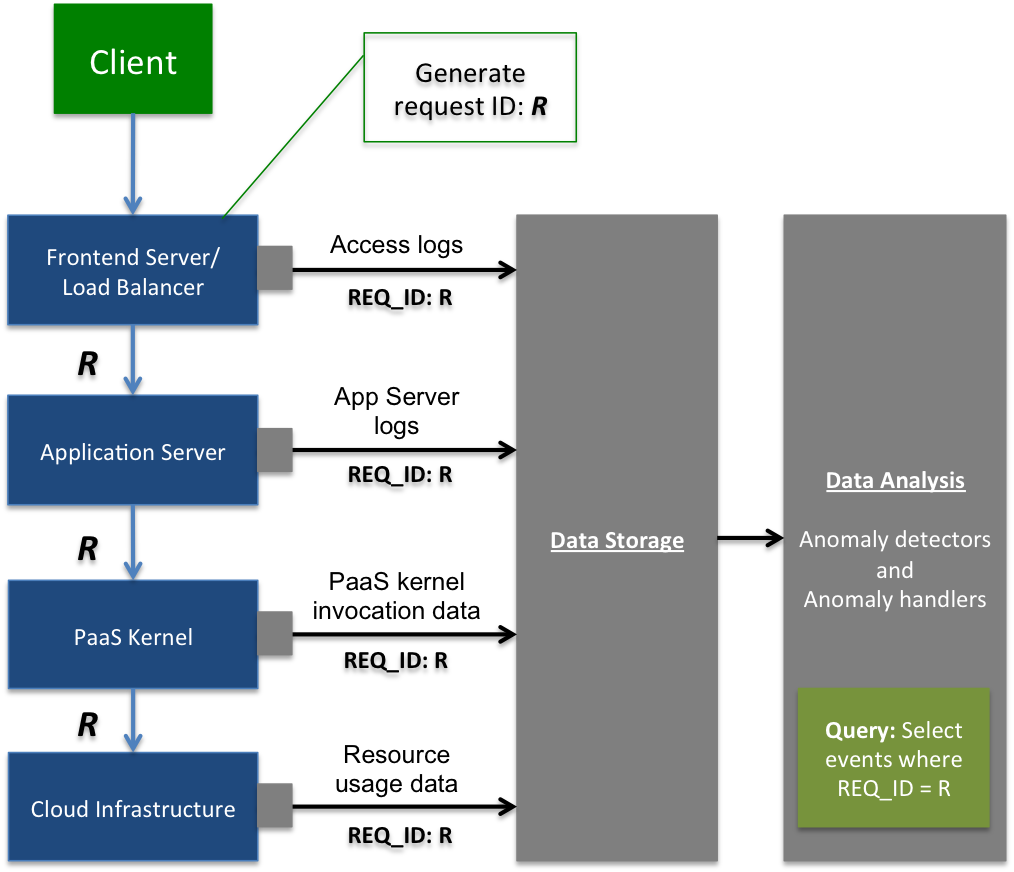
\includegraphics[scale=0.5]{apm_architecture}
\caption{Roots APM architecture.}
\label{fig:apm_architecture}
\end{figure}

Figure~\ref{fig:apm_architecture} illustrates the high-level architecture of the proposed APM, and how 
it fits into the PaaS cloud stack. APM components are shown in grey, with their interactions indicated
by the black lines. The small grey boxes attached to the PaaS components represent the sensors and
agents used to instrument the cloud platform for data collection purposes. Note that the APM collects
data from all layers in the PaaS stack (i.e. full stack monitoring).

From the front-end and load balancing layer we gather all information related to incoming application
requests. A big part of this is scraping the HTTP server access logs, which indicate request timestamps,
source and destination addressing information, response time (latency) and other HTTP message
parameters. This information is readily available for harvesting in most technologies used as front-end
servers (e.g. Apache HTTPD, Nginx). Additionally we may also collect information pertaining to active
connections, invalid access attempts and other errors.

From the application server layer we collect basic application logs as well as any other
metrics that can be easily collected from the application runtime. This may include some process level
metrics indicating the resource usage of the individual application instances. Additionally Roots
employs a set of per-application benchmarking processes, that periodically probes applications
to measure their performance. These are lightweight, stateless processes managed by the Roots framework.
Data collected by these processes will also be sent to data storage component, and will be available
for analysis as per-application timeseries data.

At the PaaS kernel layer we employ instrumentation to record information regarding all kernel invocations
made by the applications. This instrumentation must be applied carefully as to not introduce a noticeable
overhead to the application execution. For each PaaS kernel invocation, we can capture the 
following parameters.
\begin{itemize}
\item Source application making the kernel invocation
\item Timestamp
\item Target kernel service and operation
\item Execution time of the invocation
\item Request size, hash and other parameters
\end{itemize}
Collecting this PaaS kernel invocation details enables tracing the execution of application 
requests, without the need for instrumenting application code, which we believe is a feature 
unique to Roots. 

Finally, at the lowest infrastructure level, we can collect information related to virtual machines, containers
and their resource usage. We can also gather metrics on network usage by individual components which
might be useful in a number of traffic engineering use cases. Where appropriate we can also scrape
hypervisor and container manager logs to get an idea of how resources are allocated and released over
time.

To avoid introducing delays to the application request processing flow, we implement
all Roots data collecting agents as asynchronous tasks. That is, none of them would
suspend application request processing to report data to the data storage components.
We make sure that all expensive I/O tasks related to data collection and storage is
executed out of the request processing flow.
In particular, all data is collected into log files or memory buffers that are local to the components being
monitored. This locally collected (or buffered) data will be periodically sent
to the data storage components of Roots using separate background tasks and batch communication
operations. Also special care is taken to isolate the activities in the cloud from potential
faults in the Roots data collection or storage layers. 

\subsubsection{Cross-layer Data Correlation}
Previous subsection details how the APM collects useful monitoring data at each layer of the cloud
stack. To make most out of the gathered data, and use them to perform complex analyses, 
we must be able to correlate data records collected at different layers of the PaaS. For example consider
the execution of a single application request. This single event results in following data records at
different layers of the cloud, which will be collected and stored by the APM as separate entities.

\begin{itemize}
\item A front-end server access log entry
\item Zero or more application log entries
\item Zero or more PaaS kernel invocation records
\end{itemize}

We require a mechanism to tie these disparate records together, so the data processing components can easily
aggregate the related information. For instance, we must be able to retrieve via an
aggregation query, all PaaS kernel invocations made by a specific application request.

To facilitate this requirement we propose that front-end server tags all incoming application requests 
with unique identifiers.
This request identifier can be attached to HTTP requests as a header which is visible to all components 
internal to the PaaS cloud. All data collecting agents can then be configured to record the request identifiers
whenever recording an event. At the data processing layer Roots can aggregate the data by request identifiers
to efficiently group the related records.

\subsubsection{Data Analysis}
Roots data analysis component uses two basic abstractions:
\begin{itemize}
\item Anomaly detector
\item Anomaly handler
\end{itemize}

Anomaly detectors are processes that periodically analyze the data collected for
each deployed application. Roots supports multiple detector implementations, where each implementation
uses a different statistical method to look for performance anomalies. Detectors are configured
at application level making is possible for different applications to use different anomaly 
detectors. Roots also supports multiple concurrent anomaly detectors on the same application, which can be used
to evaluate the efficiency of different detection strategies for any given application. Each
anomaly detector has an execution schedule (e.g. run every 60 seconds), and a sliding window 
(e.g. from 10 minutes ago to now)
associated with it. The boundaries of the window determines the time range
of the data processed by the detector at any round of execution. Window is updated 
after each round of execution.

When an anomaly detector finds an anomaly in application performance, it sends an event
to a collection of anomaly handlers. The event encapsulates a unique anomaly identifier, 
timestamp, application identifier and the source detector's sliding window that correspond to the
anomaly. Anomaly handlers are configured globally (i.e. each handler
receives events from all detectors), but they can choose to not handle certain types
of anomalies. Similar with detectors, Roots supports multiple anomaly handler
implementations -- one for logging anomalies, one for sending alert emails, one
for updating a dashboard etc. Additionally, Roots provides two special anomaly handler
implementations: a workload change analyzer, and a root cause analyzer.

Both the anomaly detectors and anomaly handlers work with fix-sized sliding windows.
They are free to discard any old data as the sliding window moves along the time line.
As such the amount of state information these entities must keep in memory has
a strict upper bound. The old 
historical data can be kept persistently in the Roots data storage layer, until
they are deemed eligible for garbage collection.

The extensibility of Roots is primarily achieved through the abstractions of anomaly
detectors and handlers. Roots makes it simple to implement new detectors and handlers,
and plug them into the system. Both the detectors and the handlers are executed
as lightweight processes that do not interfere with the rest of the processes in
the cloud platform. Therefore failures in detectors and handlers have no impact
on the cloud platform or the deployed applications.